%% 
%% Copyright 2007-2019 Elsevier Ltd
%% 
%% This file is part of the 'Elsarticle Bundle'.
%% ---------------------------------------------
%% 
%% It may be distributed under the conditions of the LaTeX Project Public
%% License, either version 1.2 of this license or (at your option) any
%% later version.  The latest version of this license is in
%%    http://www.latex-project.org/lppl.txt
%% and version 1.2 or later is part of all distributions of LaTeX
%% version 1999/12/01 or later.
%% 
%% The list of all files belonging to the 'Elsarticle Bundle' is
%% given in the file `manifest.txt'.
%% 
%% Template article for Elsevier's document class `elsarticle'
%% with harvard style bibliographic references

%\documentclass[preprint,12pt,twocolumns]{elsarticle}

%% Use the option review to obtain double line spacing
%% \documentclass[preprint,review,12pt]{elsarticle}

%% Use the options 1p,twocolumn; 3p; 3p,twocolumn; 5p; or 5p,twocolumn
%% for a journal layout:
%% \documentclass[final,1p,times]{elsarticle}
%% \documentclass[final,1p,times,twocolumn]{elsarticle}
%% \documentclass[final,3p,times]{elsarticle}
%% \documentclass[final,3p,times,twocolumn]{elsarticle}
 \documentclass[final,5p,times]{elsarticle}
%% \documentclass[final,5p,times,twocolumn]{elsarticle}

%% For including figures, graphicx.sty has been loaded in
%% elsarticle.cls. If you prefer to use the old commands
%% please give \usepackage{epsfig}

%% The amssymb package provides various useful mathematical symbols
\usepackage{amssymb}
\usepackage[spanish]{babel}
\usepackage{listings} 
\usepackage{color}
\usepackage[small]{caption}
%% The amsthm package provides extended theorem environments
%% \usepackage{amsthm}

%% The lineno packages adds line numbers. Start line numbering with
%% \begin{linenumbers}, end it with \end{linenumbers}. Or switch it on
%% for the whole article with \linenumbers.
%% \usepackage{lineno}

%\journal{Nuclear Physics B}

\definecolor{dkgreen}{rgb}{0,0.6,0}
\definecolor{gray}{rgb}{0.5,0.5,0.5}
\definecolor{mauve}{rgb}{0.58,0,0.82}

\lstset{frame=tb,
  language=Python,
  aboveskip=3mm,
  belowskip=3mm,
  showstringspaces=false,
  columns=flexible,
  basicstyle={\small\ttfamily},
  numbers=none,
  numberstyle=\tiny\color{gray},
  keywordstyle=\color{blue},
  commentstyle=\color{dkgreen},
  stringstyle=\color{mauve},
  breaklines=true,
  breakatwhitespace=true,
  tabsize=3
}

\begin{document}

\begin{frontmatter}

%% Title, authors and addresses

%% use the tnoteref command within \title for footnotes;
%% use the tnotetext command for theassociated footnote;
%% use the fnref command within \author or \address for footnotes;
%% use the fntext command for theassociated footnote;
%% use the corref command within \author for corresponding author footnotes;
%% use the cortext command for theassociated footnote;
%% use the ead command for the email address,
%% and the form \ead[url] for the home page:
%% \title{Title\tnoteref{label1}}
%% \tnotetext[label1]{}
%% \author{Name\corref{cor1}\fnref{label2}}
%% \ead{email address}
%% \ead[url]{home page}
%% \fntext[label2]{}
%% \cortext[cor1]{}
%% \address{Address\fnref{label3}}
%% \fntext[label3]{}

\title{Violencia intrafamiliar y comunitaria en Nuevo Le\'on}

%% use optional labels to link authors explicitly to addresses:
%% \author[label1,label2]{}
%% \address[label1]{}
%% \address[label2]{}

\author{Gabriela S\'anchez Yepez}

\address{Posgrado en Ingenier\'ia de Sistemas \\
Facultad de Ingenier\'ia Mec\'anica y El\'ectrica\\
Universidad Aut\'onoma de Nuevo Le\'on}
%\ead{saphira3000@hotmail.es}

\begin{abstract}
Se presenta un an\'alisis de incidentes de violencia intrafamiliar y comunitaria en el estado de Nuevo Le\'on reportados durante el a\~no 2018. Es importante identificar los grupos vulnerables y posibles causas al problema que permitan planear estrategias de prevenci\'on. Para realizar dicho an\'alisis, se utilizan distintas herramientas que proporciona el lenguaje de programaci\'on Python. %Se busca identificar el grupo m\'as vulnerable a presentar violencia familiar as\'i c\'omo las posibles causas co el objetivo de  %Como principal objetivo se busca identificar el grupo m\'as vulnerable para planear estrategias de prevenci\'on.
\end{abstract}

%%Graphical abstract
%\begin{graphicalabstract}
%\includegraphics{grabs}
%\end{graphicalabstract}

%%Research highlights
%\begin{highlights}
%\item Research highlight 1
%\item Research highlight 2
%\end{highlights}

\begin{keyword}
%% keywords here, in the form: keyword \sep keyword

%% PACS codes here, in the form: \PACS code \sep code

%% MSC codes here, in the form: \MSC code \sep code
%% or \MSC[2008] code \sep code (2000 is the default)

\end{keyword}

\end{frontmatter}

%% \linenumbers

%% main text
%\twocolumn[
%\begin{@twocolumnfalse}
\section{Introducci\'on} \label{intro}

Este trabajo busca aplicar herramientas de ciencia de datos que permitan analizar el efecto de distintos factores presentes en incidentes de violencia intrafamiliar y comunitaria en el estado de Nuevo Le\'on, con el objetivo de identificar vulnerables y posibles causas al problema que permitan planear estrategias de prevenci\'on.

La estructura del art\'iculo es la siguiente: * 

%\section{Antecedentes} \label{antecedentes}

%\section{Literatura relacionada} \label{estado_arte}

\section{Metodolog\'ia} \label{metodologia}

En esta secci\'on se especifican las car\'acteristicas de los datos con los que se trabaja as\'i como las herramientas utilizadas para el an\'alisis de dichos datos. 

\subsection{Datos}

Los datos fueron proporcionados por la doctora Patricia L. Cerda P\'erez, en formato xlsx.

Los datos se presentan en dos archivos, el primero contiene los incidentes de violencia intrafamiliar y comunitaria presentados durante los meses de enero a noviembre en el a\~no 2018 y el segundo, los incidentes del resto del a\~no, teniendo un total de 16 410 reportes. 

Los registros contienen 47 columnas de las cuales \'unicamente 17 proporcionan informaci\'on relevante, sin datos personales, que ser\'an usados en el an\'alisis. Estos registros proveen datos sobre lugar, fecha y hora de los incidentes, as\'i como informaci\'on sobre la(s) v\'ictima(s) y agresor(es).  

\subsection{Herramientas}

En esta subsecci\'on se explica la selecci\'on de herramientas para los distintos an\'alisis que fueron realizados.

\subsubsection*{Preprocesamiento de los datos} 
Para realizar un preprocesamiento de los datos primero se utiliz\'o la herramienta \textsc{bash} que permiti\'o convertir el archivo de los datos a un formato manejable, esto es, csv, utilizando la instrucci\'on
\begin{lstlisting}
sscovert datos.xlsx vf.csv
\end{lstlisting}

La siguiente fase de preprocesamiento se realiz\'o con la librer\'ia \textsc{pandas}. El primer paso es unir los datos en un solo archivo, eliminar la informaci\'on que no se utiliza y cambiar los tipos de los datos para no tener problemas una vez que se empiece a procesar la informaci\'on.

\subsubsection*{Estad\'istica descriptiva y visualizaci\'on de la informaci\'on}

El an\'alisis estad\'istico b\'asico as\'i como una visualizaci\'on de la informaci\'on se realiz\'o con distintas herramientas proporcionadas por la librer\'ia \textsc{pandas}.

Para poder trabajar con esta librer\'ia es necesario cargar los datos para que se lean en el formato que se requiere, esto se logra con
\begin{lstlisting}
import pandas as pd
vf = pd.read_csv("vf.csv")
\end{lstlisting}

En el an\'alisis descriptivo se revisan los datos que pueden estudiarse cuantitativamente tales como la cantidad de incidentes reportados por mes, hora y fecha, entre otros. Esto se puede realizar utilizando la siguiente instrucci\'on
\begin{lstlisting}
vf.mes.value_counts(sort=True, normalize=False, dropna=True)
\end{lstlisting}
los resultados nos permiten observar el impacto de dichos factores en el total de los incidentes. 

Estos y otros resultados, tales como las edades de las v\'ictimas y agresores, pueden visualizarse gr\'aficamente utilizando la librer\'ia \textsc{plotly}. 

Para poder graficar estos datos, la informaci\'on correspondiente debe ser procesada ya que hay reportes para los cuales no se especifica la edad del agresor o la v\'ictima; en algunos casos el reporte fue llenado con un \textit{NE} y en otros casos se report\'o un rango por ejemplo \textit{40 a 45 a\~nos}. La forma en que se procede a limpiar estos datos es la siguiente
\begin{lstlisting}
edadv = vf.edad_v # edades de las victimas
edad_v = []
for dato in edadv:
    s = str(dato).replace(",", " ")
    pedazos = s.split()   
    while "a" in pedazos:
        pos = pedazos.index("a")
        desde = int(pedazos[pos - 1])
        hasta = int(pedazos[pos + 1])
        prom = (desde + hasta) // 2
        edad_v.append(prom)
        pedazos = pedazos[:(pos - 1)] + pedazos[(pos + 2):]
    edad_v += pedazos
edad_v = list(filter(lambda dato: dato != "NE", edad_v)) 
edad_v = list(filter(lambda dato: dato != "nan", edad_v))
\end{lstlisting}

Una vez que los datos est\'en en el formato adecuado se procede a graficar. Por ejemplo, teniendo la informaci\'on de las edades de las v\'ictimas y agresores en los \textit{diccionarios di\_edadA} y \textit{di\_edadV}, se puede graficar un diagrama de barras:
\begin{lstlisting}
import plotly
import plotly.plotly as py
import plotly.graph_objs as go

trace1 = go.Bar(
    x = list(di_edadA.keys()),
    y = list(di_edadA.values()),
    name = 'Edad agresores'
)
trace2 = go.Bar(
    x = list(di_edadV.keys()),
    y = list(di_edadV.values()),
    name = 'Edad victimas'
)

data = [trace1, trace2]
layout = go.Layout(
    barmode = 'group'
)
\end{lstlisting}

\subsubsection*{Modelos lineales}

Modelos lineales con scipy.stats

Modelos lineales son para representar una variable de interés como una función de uno o más factores conocidos de tal forma que se maximice la proporción de variación explicada por el modelo.



\section{Resultados} \label{resultados}

En esta secci\'on se presentan los resultados del an\'alisis y experimentos que se realizan.

Primero se muestran gr\'aficos que permiten una visualizaci\'on de la informaci\'on con la que se trabaja. 

Las Figuras \ref{incidentes_horas} y \ref{indicentes_mes} muestran un histograma de la cantidad de incidentes reportados de acuerdo a las horas y de acuerdo a los meses respectivamente. De ellas podemos observar que el rango de horarios de las 20:00 - 01:00 horas es el que reporta una mayor cantidad de incidentes mientras que en el caso de los meses, julio fue el mes m\'as violento de ese a\~no.

\begin{figure}
\centering
\includegraphics[scale=0.6]{horas.eps}
\caption{Cantidad de incidentes reportados por hora durante el a\~no 2018.}
\label{incidentes_horas}
\end{figure} 

\begin{figure}
\centering
\includegraphics[scale=0.6]{mes.eps}
\caption{Cantidad de incidentes reportados por mes durante el a\~no 2018.}
\label{indicentes_mes}
\end{figure} 

Para visualizar el rango de edades de v\'ictimas y agresores, primero se agrupan en d\'ecadas para evitar obtener \textit{peines} por la falta de informaci\'on reportada. La Figura \ref{edades} muestra la gr\'afica que corresponde a esta informaci\'on. De esta figura se resalta la cantidad de incidentes con v\'icimas entre 0-10 a\~nos pues se reportan 922 casos, adem\'as se reportan 111 casos de v\'ictimas mayores de 80 a\~nos. 

Tambi\'en es notorio que la mayor\'ia de los incidentes ocurre con agresores y v\'ictimas de edades de 30-50 a\~nos. 
\begin{figure}
\centering
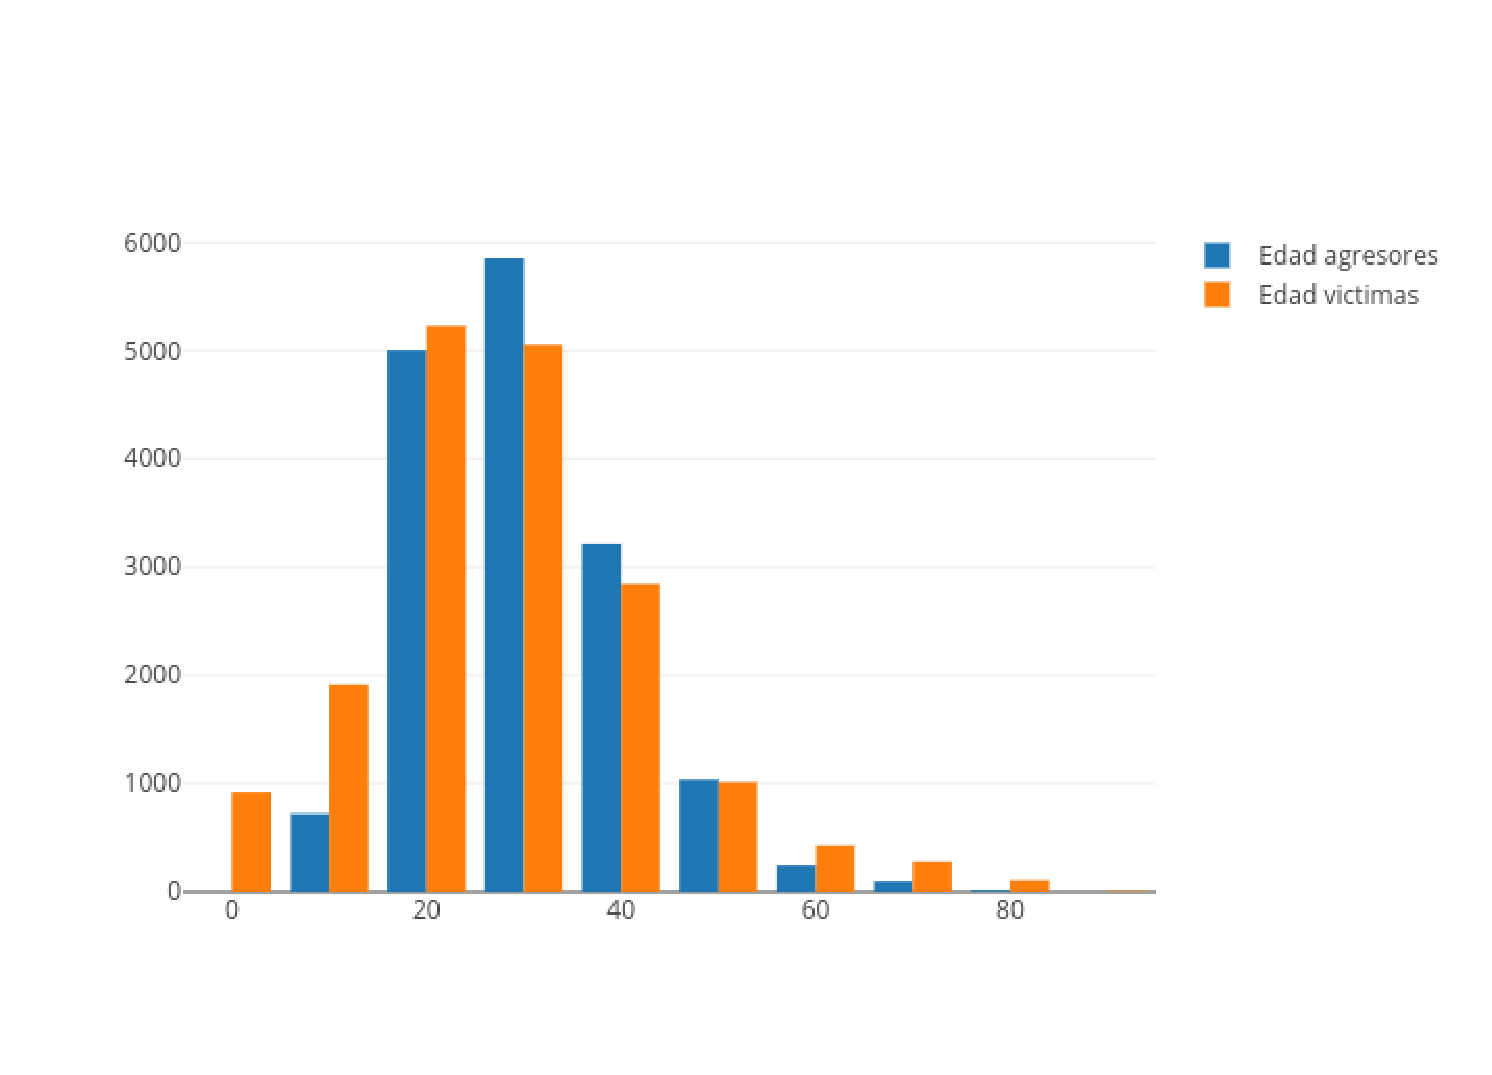
\includegraphics[scale=0.4]{edades.eps}
\caption{Rango de edades de v\'ictimas y agresores.}
\label{edades}
\end{figure} 



\section{Conclusiones} \label{conclusiones}

%% The Appendices part is started with the command \appendix;
%% appendix sections are then done as normal sections
%% \appendix

%% \section{}
%% \label{}

%% For citations use: 
%%       \citet{<label>} ==> Jones et al. [21]
%%       \citep{<label>} ==> [21]
%%

%% If you have bibdatabase file and want bibtex to generate the
%% bibitems, please use
%%
%%  \bibliographystyle{elsarticle-num-names} 
%%  \bibliography{<your bibdatabase>}

%% else use the following coding to input the bibitems directly in the
%% TeX file.

\begin{thebibliography}{00}

%% \bibitem[Author(year)]{label}
%% Text of bibliographic item

%\bibitem[ ()]{}

\end{thebibliography}

\section*{Agradecimientos}

Agradezco al Consejo Nacional de Ciencia y Tecnolog\'ia (CONACyT) por la beca otorgada. A la doctora Patricia L. Cerda P\'erez por proveer los datos utilizados en el estudio y a la doctora Elisa Schaeffer por la gu\'ia proporcionada para la realizaci\'on de este trabajo.


%\end{@twocolumnfalse}]
\end{document}

\endinput
%% End of file `elsarticle-template-num-names.tex'.
